\documentclass[main.tex]{subfiles}
\begin{document}

\section{Limieten van rijen in $\mathbb{R}^{p}$.}
\label{cha:cont-voor-funct}

\begin{de}
  De verzameling $\mathbb{R}^{p}$ met $p\in \mathbb{N}_{0}$ definieren we als volgt:
  \[ \left\{ (q_{1},q_{2},\dotsc,q_{p}) \mid \forall i \in \{1,2,\dotsc,p\}: q_{i}\in \mathbb{R} \right\} \]
\end{de}

\begin{de}
  We definieren het \term{product} van een element $q\in \mathbb{R}^{p}$ met een element $\lambda\in \mathbb{R}$ als volgt:
  \[ \lambda q = \lambda (q_{1},q_{2},\dotsc,q_{p}) = (\lambda q_{1},\lambda q_{2},\dotsc,\lambda q_{p}) \]
\end{de}

\begin{de}
  We definieren het \term{scalair product} $\langle v,w \rangle$ van twee elementen $v,w\in \mathbb{R}^{p}$ definieert men als volgt:
  \[ \langle v,w \rangle = \sum_{i=0}^{p}v_{i}w_{i} \]
\end{de}

\begin{de}
  We definieren de \term{norm} van een element $v\in \mathbb{R}^{q}$ als de wortel van het scalair product met zichzelf:
  \[ \|v\| = \sqrt{\langle v,v \rangle} = \sum_{i=0}^{p}v_{i}^{2} \in \mathbb{R} \]
\end{de}

\begin{de}
  We definieren de \term{afstand} $d(v,w)$ tussen twee elementen $v,w \in \mathbb{R}^{p}$ als volgt:
  \[ d(v,w) = \|v-w\| \in \mathbb{R} \]
\end{de}

\begin{st}
  \label{st:eerste-driehoeksongelijkheid-rp}
  Voor die afstand geldt de driehoeksongelijkheid:
  \[ \|a+b\| \le \|a\| + \|b\| \]
\extra{bewijs}
\end{st}

\begin{st}
  \label{st:tweede-driehoeksongelijkheid-rp}
  Voor die afstand geldt de tweede driehoeksongelijkheid:
  \[ \|v-w\| \le \|v-z\| + \|z-w\| \]
\extra{bewijs}
\end{st}

\begin{st}
  Er is geen 'natuurlijke orde' in $\mathbb{R}^{p}$.
\clarify{wat betekent dit zelfs?}
\end{st}

\subsection{Rijen in $\mathbb{R}^p$}
\label{sec:rijen-mathbbrp}

\begin{de}
  We noemen een rij $(x_{n})_{n}$ in $\mathbb{R}^{p}$ \term{convergeert} naar een $q\in \mathbb{R}^{p}$ als en slechts als het volgende geldt:
  \[ \forall \epsilon \in \mathbb{R}_{0}^{+}, \exists n_{0}\in \mathbb{N}, \forall n\in \mathbb{N}:\ n\ge n_{0} \Rightarrow \|x_{n}-q\| < \epsilon  \]
  We noteren dit als volgt:
  \[ \lim_{n\rightarrow +\infty}x_{n} = q \]
\end{de}

\begin{opm}
  Het concept van een oneindige limiet bestaat niet op dezelfde manier.
  We kunnen enkel componentsgewijs over limieten naar oneindig spreken, of aan de hand van de norm.
\extra{doen? of niet nuttig?}
\end{opm}

\begin{st}
  \label{st:in-rp-convergeert-asa-componenten-convergeren}
  Zij $(x_{n})_{n} = ((x_{1,n},x_{2,n},\dotsc,x_{p,n})_{n}$ een rij in $\mathbb{R}^{p}$, dan convergeert $(x_{n})$ als en slechts als elk van de rijen $(x_{i,n})_{n}$ convergeert.

  \begin{proof}
    Zij $x$ de limiet van $(x_{n})_{n}$.
    Merk de volgende ongelijkheden op:\stref{st:eerste-driehoeksongelijkheid-rp}\stref{st:tweede-driehoeksongelijkheid-rp}
    \begin{align*}
      \|x_{n}-x\| &\le |x_{n,1}-x_{1}| + |x_{n,2}-x_{2}| + \dotsc + |x_{n,p}-x_{p}|\\
      |x_{n,i}-x_{i}| &\le \|x_{n}-x\|
    \end{align*}
    \begin{itemize}
    \item $\Rightarrow$\\
      Kies willekeurig een $\delta \in \mathbb{R}_{0}^{+}$ en een willekeurige $i$.
      Omdat er een $n_{0}$ bestaat zodat $x_{n}$ dichter dan $\delta$ bij $x$ komt, en de afstand van $x_{n,i}$ tot $x_{i}$ kleiner is dan, of gelijk aan, de afstand tusssen $x_{n}$ en $x$, kunnen we diezelfde $n_{0}$ nemen om $x_{n,i}$ willekeurig dicht bij $x_{i}$ te laten komen.
    \item $\Leftarrow$\\
      Kies willekeurig een $\delta \in \mathbb{R}_{0}^{+}$.
      Voor elke $i$ bestaat er een $n_{i}$ zodat $x_{n,i}$ dichter dan $\frac{\delta}{p}$ bij $x_{i}$ komt.
      Neem nu $m=\max_{i}\{x_{i}\}$, dan komt $x_{n}$ dichter dan $p\frac{\delta}{p}=\delta$ bij $x$.
    \end{itemize}
  \end{proof}
\end{st}

\begin{st}
  Een limiet van een rij, als hij bestaat, is uniek.

  \begin{proof}
    Stel dat een rij $(x_{n})_{n}$ in $\mathbb{R}^{p}$ twee limieten $a$ en $b$ in $\mathbb{R}^{p}$ heeft.
    \[ \lim_{n\rightarrow +\infty}x_{n} = a \quad\text{ en }\quad \lim_{n\rightarrow +\infty}x_{n} = b \]
    Noem nu $\delta = \frac{1}{2}\|a-b\|$.
    Omdat $a$ de limiet is van $(x_{n})_{n}$ bestaat er een $n_{a} \in \mathbb{N}$ als volgt:
    \[ \forall n\in \mathbb{N}:\ n \ge n_{a} \Rightarrow \|x_{n}-a\| < \delta \]
    Omdat $b$ ook de limiet is van $(x_{n})_{n}$ bestaat ook er een $n_{b} \in \mathbb{N}$ als volgt:
    \[ \forall n\in \mathbb{N}:\ n \ge n_{b} \Rightarrow \|x_{n}-b\| < \delta \]
    Omdat $a$ en $b$ een afstand $2\delta$ uit elkaar liggen moeten de volgende verzamelingen $A$ en $B$ disjunct zijn.

    \noindent
    \begin{minipage}{.45\textwidth}
      \begin{figure}[H]
        \centering
        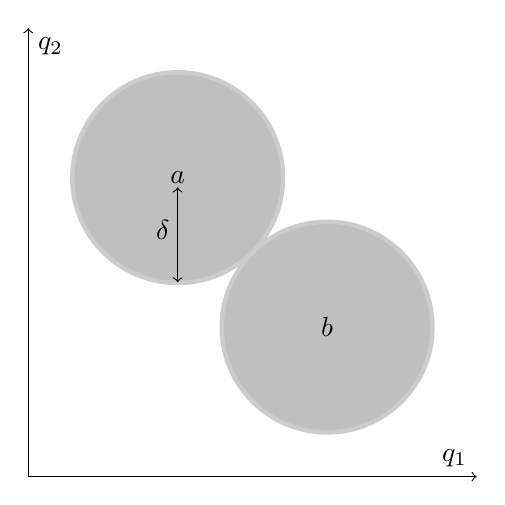
\begin{tikzpicture}
          \begin{axis}[ 
            ticks=none,
            axis lines = middle,
            axis line style={->},
            ymin=0, ymax=3,
            xmin=0, xmax=3,
            xlabel={$q_{1}$},
            ylabel={$q_{2}$},
            axis equal image,
            disabledatascaling
            ]
            \filldraw[fill=black!25!white, draw=black!20!white,ultra thick] (1,2) circle [radius=.705];
            \filldraw [fill=black!25!white, draw=black!20!white,ultra thick] (2,1) circle [radius=.705];
            \draw (1,2) node {$a$};
            \draw (1,2) node {} edge[<->] (1,1.3);
            \draw (.9,1.65) node {$\delta$};
            \draw (2,1) node {$b$};
            
          \end{axis}
        \end{tikzpicture}
        \caption{Illustratie in $\mathbb{R}^{2}$}
      \end{figure}
    \end{minipage}
    \begin{minipage}{.45\textwidth}
      \[ A = \{ q \in \mathbb{R}^{p} \mid \|q-a\| < \delta \} \]
      \[ B = \{ q \in \mathbb{R}^{p} \mid \|q-b\| < \delta \} \]
    \end{minipage}
    
    \noindent
    Neem immers een getal $q$ dat in $A \cap B$ zou zitten, dan moet er het volgende gelden volgens de driehoeksongelijkheid:\stref{st:driehoeksongelijkheid-rp}
    \[ d(a,b) \le d(a,q) + d(q,b) \]
    Dit is in contradictie met het feit dat $d(a,b)$ gelijk is aan $2\delta$ en dat $d(a,q)$ en $d(q,b)$ beide strikt kleiner zijn dan $\delta$.
    Kies nu een $m\in \mathbb{N}$, groter dan zowel $n_{a}$ als $n_{b}$, dan geldt het volgende:
    \[ \forall n \in \mathbb{N}:\ n \ge m \Rightarrow x_{n} \in A \cap B \]
    Dit kan niet omdat $A\cap B$ leeg is.
    Contradictie.
  \end{proof}
\feed
\end{st}

\begin{de}
  We noemen een rij \term{begrensd} als er een $M \in \mathbb{R}^{+}$ bestaat als volgt:
  \[ \forall n \in \mathbb{N}:\ \|x_{n}\| \le M \]
  We noemen $(x_{n})_{n}$ dan begrensd door $M$.
\end{de}

\begin{st}
  \label{st:in-rp-convergent-dan-begrensd}
  Een convergente rij $(x_{n})_{n}$ is begrensd.

  \begin{proof}
    Zij $(x_{n})_{n}$ een convergente rij en noem $a$ de limiet ervan.
    Er bestaat nu een $n_{a}$ als volgt:
    \[ \forall n \in \mathbb{N}:\ n \ge n_{a}:\ \|x_{n}-a\| < 1 \]
    Merk nu het volgende op:
    \[ \forall n \in \mathbb{N}:\ \|x_{n}\| = \|(x_{n}-a) + a\| \le \|x_{n}-a\| + \|a\| < \|a\|+1 \]
    \begin{figure}[H]
      \centering
      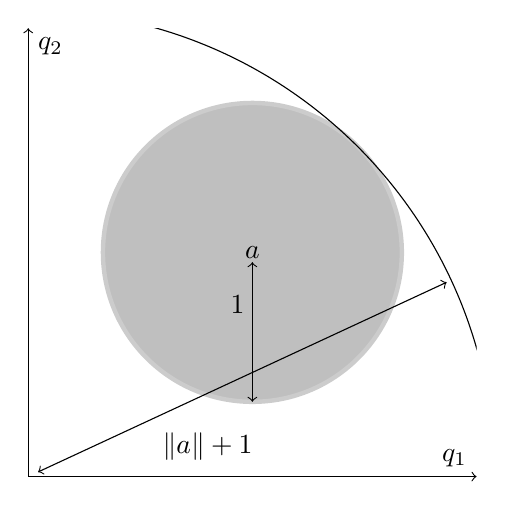
\begin{tikzpicture}
        \begin{axis}[ 
          ticks=none,
          axis lines = middle,
          axis line style={->},
          ymin=0, ymax=3,
          xmin=0, xmax=3,
          xlabel={$q_{1}$},
          ylabel={$q_{2}$},
          axis equal image,
          disabledatascaling
          ]
          \filldraw[fill=black!25!white, draw=black!20!white, ultra thick] (1.5,1.5) circle [radius=1];
          \draw (1.5,1.5) node {$a$};
          \draw (1.5,1.5) node {} edge[<->] (1.5,0.5);
          \draw (1.4,1.15) node {$1$};
          \draw[draw=black] (0,0) circle [radius=3.12];
          \draw (0,0) node {} edge[<->] (2.8,1.3);
          \draw (1.2,0.2) node {$\|a\|+1$};
        \end{axis}
      \end{tikzpicture}
      \caption{Illustratie in $\mathbb{R}^{2}$}
    \end{figure}
    Noem nu $M = \max \{ \|x_{0}\|, \|x_{1}\|, \dotsc, \|x_{n_{a}-1}\|, 1+\|a\|\}$.
    Per constructie is $(x_{n})_{n}$ nu begrensd door $M$.
  \end{proof}
\end{st}

\begin{gst}
  De omgekeerde stelling geldt niet.
\end{gst}

\begin{pr}
  Twee rijen met de volgende eigenschap hebben hetzelfde convergentiegedrag.
  \[ \exists k\in \mathbb{N}, \forall n \in \mathbb{N}:\ x_{n} = y_{n} \]

  \begin{proof}
    Bewijs uit het ongerijmde: Stel dat $(x_{n})_{n}$ een limiet $a\in\mathbb{R}^{p}$ heeft en $(y_{n})_{n}$ geen limiet.\\
    Omdat $(y_{n})_{n}$ geen limiet heeft bestaat er een $\delta$ als volgt:
    \[ \forall n_{b}\in \mathbb{N},\exists n\in \mathbb{N}:\ n \ge n_{b} \wedge\|y_{n}-a\| \ge \delta \]
    Omdat $a$ de limiet is van $(x_{n})_{n}$ bestaat er een $n_{a}\in \mathbb{N}$ als volgt:
    \[ \forall n\in \mathbb{N}:\ n\ge n_{a} \Rightarrow \|x_{n}-a\| <\delta \]
    Kies nu $m = \max\{k,n_{a}\}$, dan is $\|x_{m}-a\|$ kleiner dan $\delta$, maar geldt ook het volgende:
    \[ \|x_{m}-a\| = \|y_{m}-a\| \ge \delta \]
    Contradictie.
\feed
  \end{proof}
\end{pr}

\mst{Voor elk element $x\in \mathbb{R}^{p}$, bestaat er een rij $(q_{n})_{n}\in \mathbb{Q}^{p}$ die convergeert naar $x$.}


\begin{st}
  Zij $(x_{n})_{n}$ een convergente rij in $\mathbb{R}^{p}$.
  \[ \lim_{n\rightarrow +\infty}\lambda x_{n} = \lambda \lim_{n\rightarrow +\infty}x_{n} \]
\extra{bewijs op definitie.}
\extra{Bewijs op $\mathbb{R}$}
\end{st}

\begin{st}
  Zij $(x_{n})_{n}$ en $(y_{n})_{n}$ twee convergente rijen in $\mathbb{R}^{p}$.
  \[ \lim_{n\rightarrow +\infty}(x_{n}+y_{n}) = \lim_{n\rightarrow +\infty}x_{n}+\lim_{n\rightarrow +\infty}y_{n} \]
\extra{bewijs op definitie.}
\extra{Bewijs op $\mathbb{R}$}
\end{st}

\begin{opm}
  De vermenigvuldiging en deling van twee $p$-tallen zijn niet gedefinieerd.
\end{opm}

\begin{st}
  \label{st:in-rp-deelrij-zelfde-limiet}
  Deelrijen van convergente rijen in $\mathbb{R}^{p}$ zijn convergent en hebben dezelfde limiet.
  \extra{bewijs: triviaal?}
\end{st}

\begin{st}
  De \term{stelling van Bolzano-Weierstra\ss} (rijen).\\
  Elke begrensde rij in $\mathbb{R}^{p}$ heeft een convergente deelrij.
\extra{bewijs adhv argument voor $\mathbb{C}$}
\end{st}

\begin{de}
  Een \term{Cauchyrij} in $\mathbb{R}^{p}$ is een rij $(x_{n})_{n}$ met de volgende eigenschap:
  \[ \forall \epsilon \in \mathbb{R}_{0}^{+}, \exists n_{0}\in \mathbb{N}, \forall n,m \in \mathbb{N}:\ n,m \ge n_{0} \Rightarrow |x_{n}-x_{m}| < \epsilon \]
\end{de}

\begin{st}
  Zij $(x_{n})_{n}$ een rij in $\mathbb{R}^{p}$, dan convergeert $(x_{n})_{n}$ als en slechts als $(x_{n})_{n}$ een Cauchyrij is.
\extra{bewijs adhv argumnet voor $\mathbb{C}$, dus vanuit $\mathbb{R}$.}
\end{st}


\mst{convergentie asa cauchy}

\end{document}

%%% Local Variables:
%%% mode: latex
%%% TeX-master: t
%%% End:
